\documentclass{article}
\usepackage{graphicx}
\usepackage[T1]{fontenc}

\title{Forecasting Road Safety: Harnessing Weather Data to Predict Car Accidents}

\author{Gunnar Þrastarson, Sigurdur Haukur Birgisson, and Tómas Blær}
\date{May 2023}

\begin{document}

\maketitle
\tableofcontents

\section{Introduction}

Car accidents have devastating consequences, causing numerous fatalities and injuries worldwide. Understanding the factors that contribute to these accidents is crucial for devising effective preventive measures. Weather conditions have been identified as a significant factor influencing accident rates, and the ability to predict accidents based on current weather conditions holds the potential to mitigate risks and enhance road safety. This research aims to investigate whether it is possible to predict the average amount of car accidents in Iceland based on current weather conditions.

The importance of predicting car accidents based on weather conditions lies in the potential to implement proactive measures and provide timely warnings to drivers about hazardous conditions. By leveraging machine learning techniques, it is possible to develop models that utilize weather data to forecast accident rates. However, a key challenge faced in this research is the availability of historical weather data that includes the necessary variables for prediction.

The research primarily focuses on temperature as a weather variable, given its known impact on driving conditions and accident occurrence. Historical temperature data from the Icelandic Meteorological Office \cite{isl_weather_data} is utilized to analyze the relationship between temperature and car accidents in Iceland. However, it is important to note that the available historical weather data for Iceland does not include wind speed, another influential factor affecting driving conditions and accidents.

To address this limitation and provide a proof of concept, an additional model is trained using a comprehensive dataset from the United States \cite{usa_data}. This dataset includes not only temperature but also wind speed measurements recorded at the time of each car accident. By incorporating both temperature and wind speed in the model, it allows for an assessment of their combined influence on accident rates. This model trained on the USA dataset serves as a validation of the approach and provides insights into the predictive capabilities of incorporating multiple weather variables.

The geographical scope of this research covers Iceland and the United States, representing two distinct regions with different weather patterns and driving environments. By comparing the results between these two regions, the research aims to identify common trends and assess the transferability of the predictive models.

It is important to acknowledge the limitations of this study. The analysis is constrained by the unavailability of wind speed data for Iceland, limiting the evaluation of the complete relationship between weather conditions and accident rates. Additionally, the training data is limited to the time period between 2009 and 2022, which may not capture long-term trends or specific temporal patterns. Despite these limitations, this study serves as an initial exploration into the predictive capabilities of weather conditions on car accidents in Iceland.

In summary, this research investigates the feasibility of predicting the average amount of car accidents in Iceland based on current weather conditions. Despite the absence of wind speed data in the historical weather dataset for Iceland, a proof of concept is provided by training a model using temperature and wind speed data from the United States. By addressing these research objectives, this study aims to contribute to the understanding of the relationship between weather conditions and accident rates, enabling the development of proactive strategies to enhance road safety.

\newpage
\section{Methodology}

The methodology employed in this research study involves data collection, data preprocessing, and the utilization of machine learning techniques to predict the average amount of car accidents based on weather conditions. Two datasets, the Iceland Dataset and the USA Dataset \cite{usa_data}, were utilized for this purpose.

\subsection{Data Collection}

The first dataset, the Iceland Dataset, consisted of temperature data obtained from the Icelandic Meteorological Office \cite{isl_weather_data}. This dataset contained monthly temperature measurements from multiple weather stations across Iceland. However, the historical weather data only provided information on temperature and rainfall, with no data on wind speed. Therefore, for the Iceland analysis, the average amount of car accidents per month was used as a dependent variable, while the average temperature for each month was considered as an independent variable. The car accident data was sourced from the Icelandic Road and Coastal Administration, spanning the period from 2009 to 2022 \cite{isl_accident_data}.

The second dataset, the USA Dataset \cite{usa_data}, provided more detailed information. It included temperature and wind speed data recorded at the time of each car accident. This dataset, obtained from Kaggle, consisted of over 2.8 million data points from 2016 to 2021, covering 49 states in the USA \cite{usa_data}.

\subsection{Data Preprocessing}

To prepare the datasets for analysis, specific data preprocessing steps were undertaken.

For the Iceland Dataset, the average temperature for each month was calculated by aggregating the temperature measurements from all the weather stations across Iceland. Similarly, the average amount of car accidents per month was determined based on the available data. The two datasets were then merged to create a unified dataset for the Iceland analysis, and split into training and testing sets, with 80\% of the data used for training and 20\% for testing.

Regarding the USA Dataset, data points that did not contain temperature and wind speed information were removed from the dataset. Additionally, the temperature values were converted from Fahrenheit to Celsius, while wind speed measurements were converted from miles per hour (mph) to meters per second (m/s). Each car accident instance was categorized based on the weather conditions at the time of the accident, including temperature and wind speed. The Categorization can be seen in Table \ref{table:weather_conditions}. The dataset was then split into training and testing sets, with 80\% of the data used for training and 20\% for testing.

\begin{table}[!ht]
    \centering
    \caption{Weather Conditions Categorization} \label{table:weather_conditions}
    \begin{tabular}{ll|ll}
        \hline
        Temp. Range       & Label          & Wind Speed Range   & Label          \\ \hline
        -$\infty$ to -5°C & Extremely Cold & 0 to 2 m/s         & No Wind        \\
        -5 to 0°C         & Very Cold      & 2 to 4 m/s         & Very Low       \\
        0 to 5°C          & Cold           & 4 to 6 m/s         & Low            \\
        5 to 10°C         & Slightly Cold  & 6 to 8 m/s         & Slightly Low   \\
        10 to 15°C        & Moderate Cold  & 8 to 10 m/s        & Moderate Low   \\
        15 to 20°C        & Moderate Hot   & 10 to 12 m/s       & Moderate High  \\
        20 to 25°C        & Slightly Hot   & 12 to 14 m/s       & Slightly High  \\
        25 to 30°C        & Hot            & 14 to 16 m/s       & High           \\
        30 to 35°C        & Very Hot       & 16 to 18 m/s       & Very High      \\
        35 to $\infty$°C  & Extremely Hot  & 18 to $\infty$ m/s & Extremely High \\ \hline
    \end{tabular}
\end{table}

\subsection{Statistical Analysis}

Before applying machine learning techniques, statistical analysis was performed to understand the relationship between weather conditions and car accidents. This analysis aimed to identify any trends or patterns in the data and determine the predictive capabilities of the models.

The amount of car accidents was plotted against time to see if there were any temporal patterns. Turns out there was a clear seasonal pattern, with more accidents occurring during the winter months. Additionally, the average amount of car accidents per month was plotted against temperature to visualize the relationship between these two variables. These plots are presented in Figures \ref{fig:accidents_per_month} and \ref{fig:accidents_vs_temp}.


\begin{figure}[h!]
    \centering
    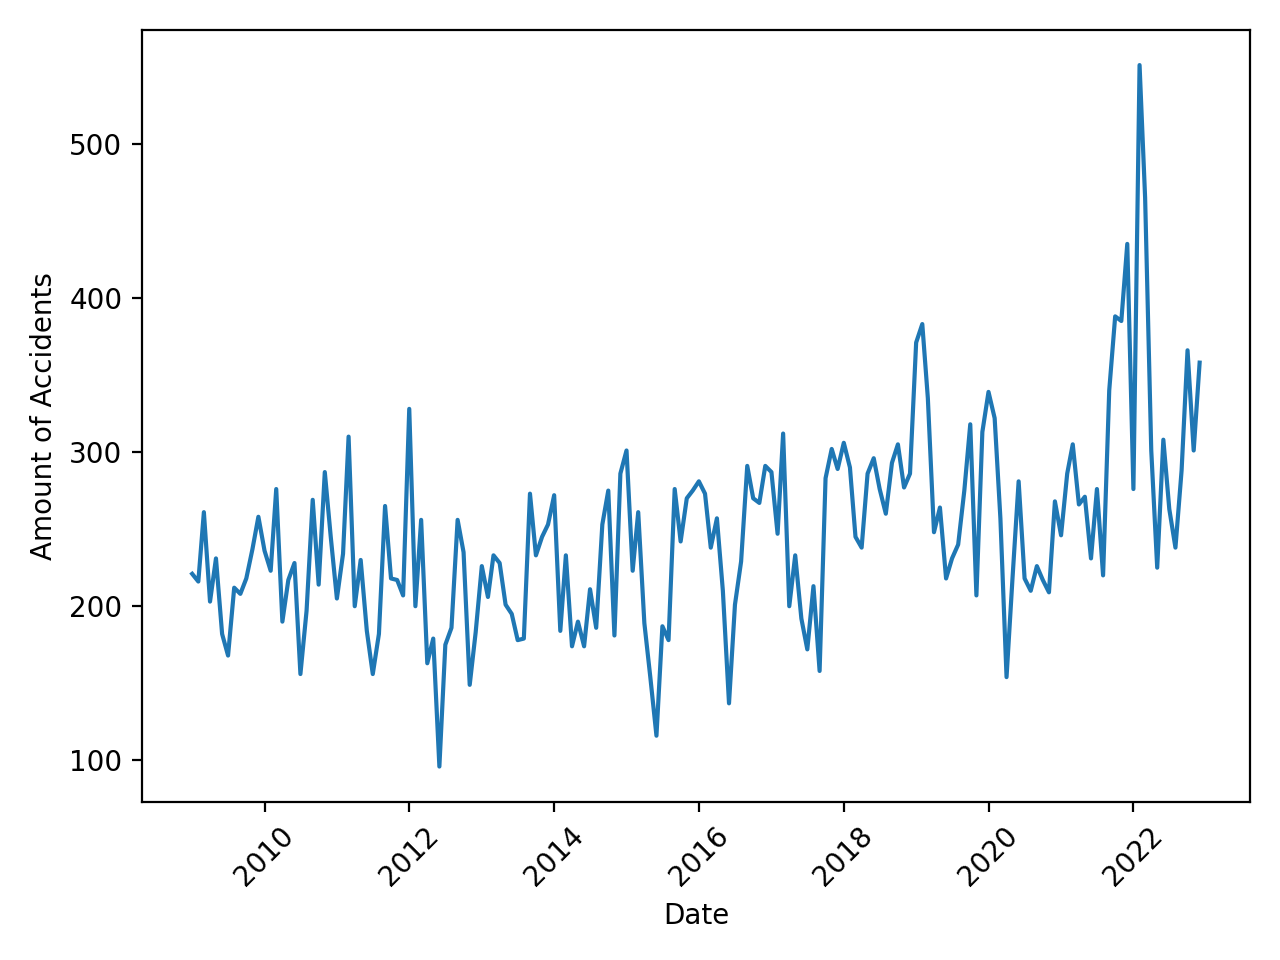
\includegraphics[scale=0.5]{../figures/highres/isl_accidents_over_time.png}
    \caption{Amount of Car Accidents per Month in Iceland}
    \label{fig:accidents_per_month}
\end{figure}

\begin{figure}[h!]
    \centering
    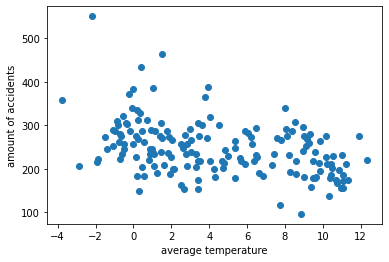
\includegraphics[scale=0.5]{../figures/highres/isl_accidents_against_temp.png}
    \caption{Amount of Car Accidents vs. Temperature in Iceland}
    \label{fig:accidents_vs_temp}
\end{figure}


There is a correlation between the amount of car accidents and temperature, with more accidents occurring at lower temperatures. However, it is important to note that the data points are spread out, indicating a high degree of variance or noise. This variance is likely due to the limited amount of data available, as well as the presence of other factors that influence accident rates, such as road conditions and driver behavior.

The same trend can be seen for the USA Dataset, but clearer. Since, it has more data points. The plots for the USA Dataset are presented in Figures \ref{fig:usa_accidents_over_time} and \ref{fig:usa_accidents_vs_temp}.

\begin{figure}[h!]
    \centering
    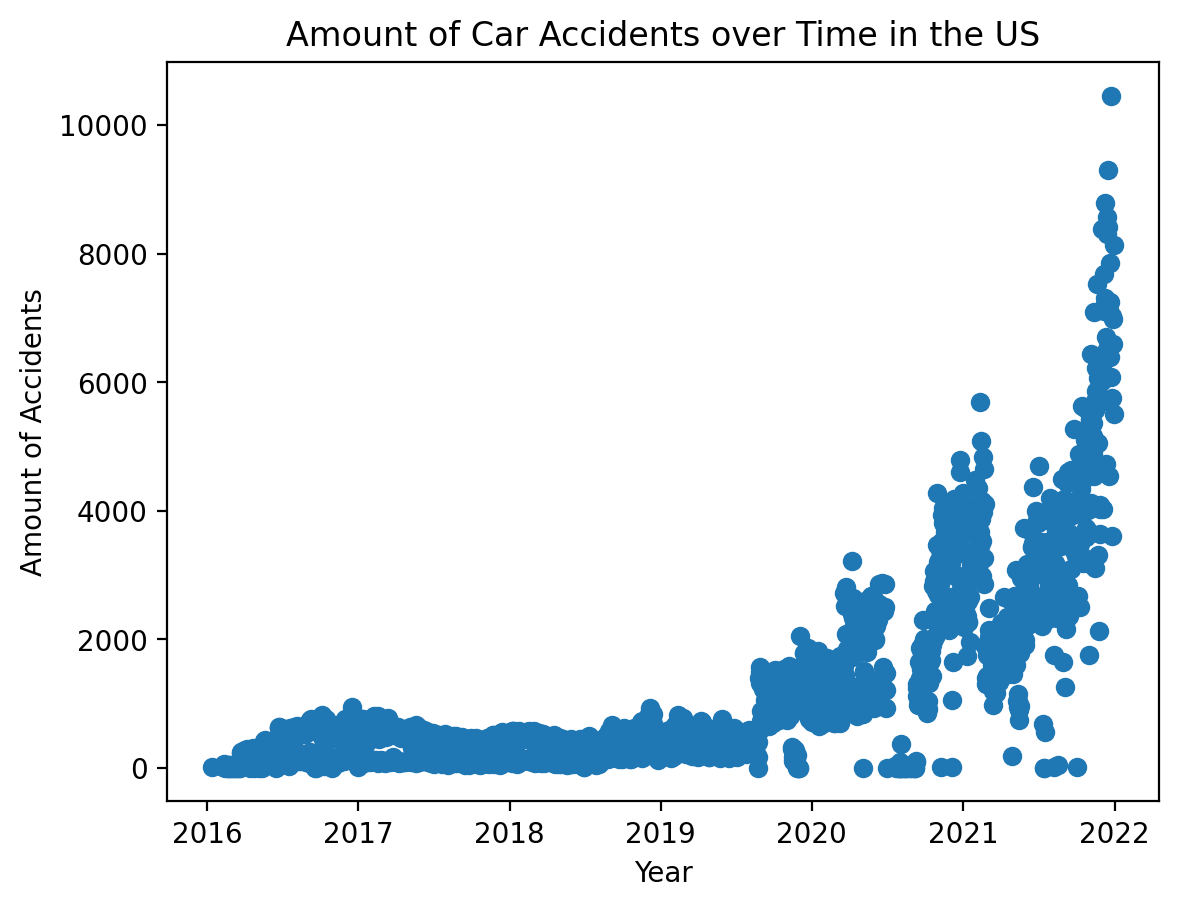
\includegraphics[scale=0.5]{../figures/highres/usa_accidents_over_time.png}
    \caption{Amount of Car Accidents per Month in the US}
    \label{fig:usa_accidents_over_time}
\end{figure}


\begin{figure}[h!]
    \centering
    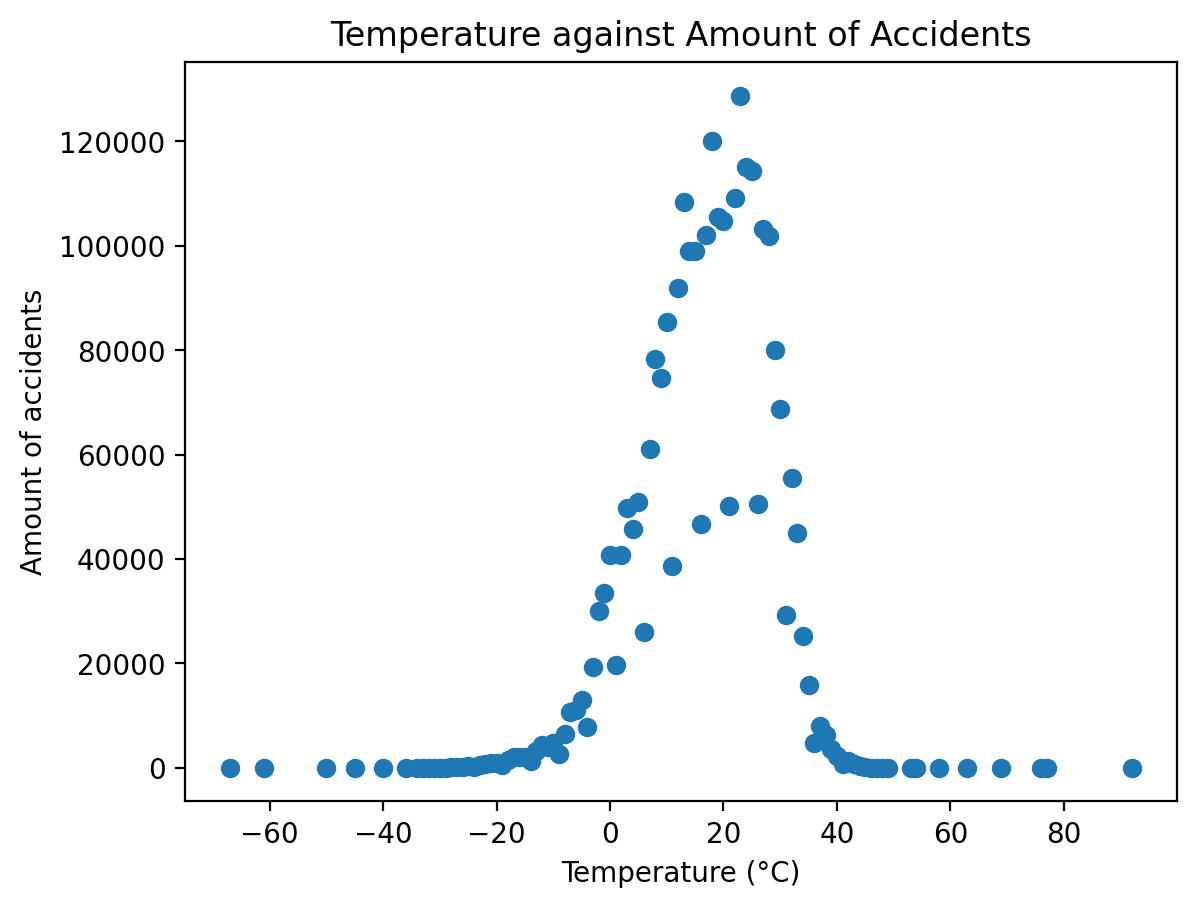
\includegraphics[scale=0.5]{../figures/highres/usa_temp_against_accidents.png}
    \caption{Amount of Car Accidents vs. Temperature in the US}
    \label{fig:usa_accidents_vs_temp}
\end{figure}

It is important to  note that most accidents in the US, occur at temperatures around 20 degrees. Because, many of the accidents happen in urban areas where there is a lot of traffic. This is also present in the Iceland Dataset, but not as clear. This is likely due to the limited amount of data available for Iceland, and the fact that there is less traffic in Iceland.

As mentioned before, the USA Dataset also included wind speed data. Therefore, the relationship between wind speed and car accidents was also examined. The amount of car accidents was plotted against wind speed to visualize the relationship between these two variables. This plot is presented in Figure \ref{fig:usa_accidents_vs_wind}.

\begin{figure}[h!]
    \centering
    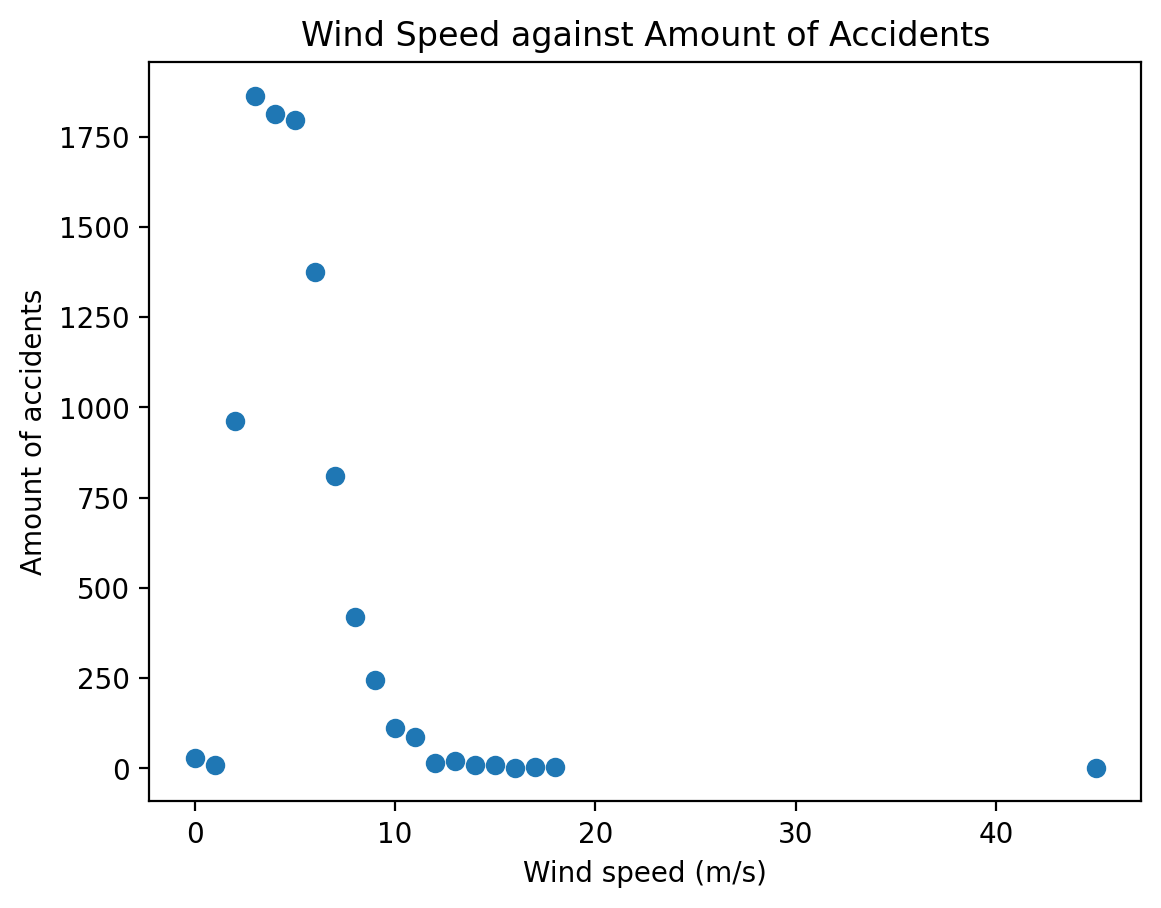
\includegraphics[scale=0.5]{../figures/highres/usa_wind_against_accidents.png}
    \caption{Amount of Car Accidents vs. Wind Speed in the US}
    \label{fig:usa_accidents_vs_wind}
\end{figure}


The plot indicates a slight correlation between wind speed and car accidents, with more accidents occurring at higher wind speeds. However, there is a limited amount of data available for the higher wind speeds. It seems that most accidents occur at wind speeds below 10 m/s. This is likely due to the fact that most accidents occur in urban areas where there is less wind.

Visualizing the effect of temperature and wind speed on car accidents at the same time is difficult. Therefore, a heatmap was created to visualize the relationship between these three variables. This heatmap is presented in Figure \ref{fig:usa_heatmap}.

\begin{figure}
    \centering
    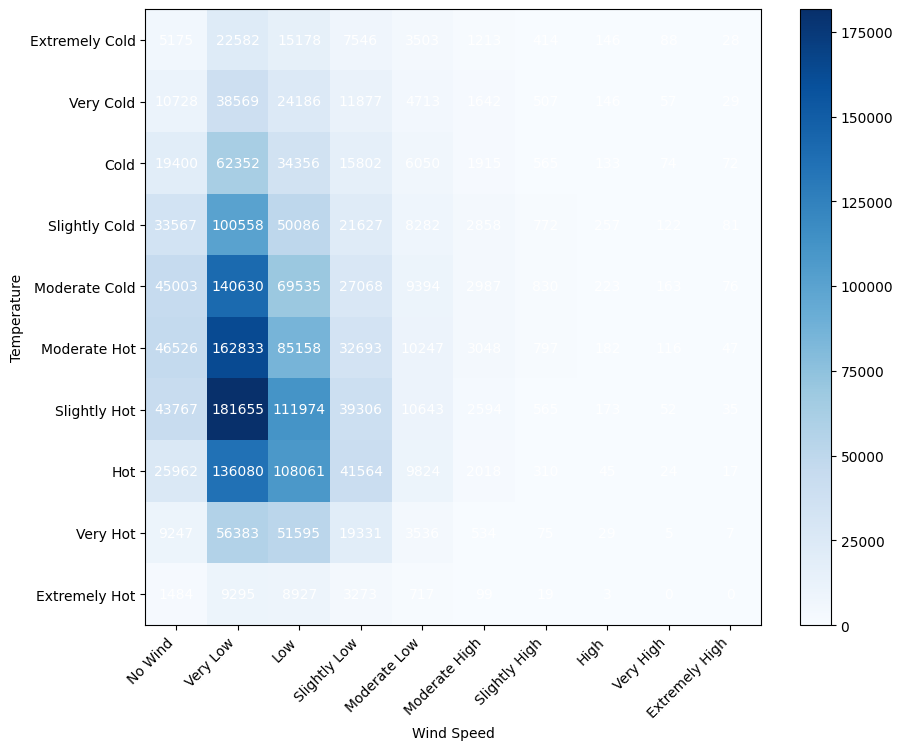
\includegraphics[scale=0.4]{../figures/highres/usa_heatmap.png}
    \caption{Heatmap of Car Accidents vs. Temperature and Wind Speed in the US}
    \label{fig:usa_heatmap}
\end{figure}

The heat map further consolidates the findings from the previous plots. It indicates that most accidents occur at temperatures around 20 degrees and wind speeds below 10 m/s. This is likely due to the fact that most accidents occur in urban areas where weather conditions have less effect.

Overall, weather conditions correlate with car accidents. However, the relationship is not very strong. This is likely due to the limited amount of data available, as well as the presence of other factors that influence accident rates, such as road conditions and traffic.


\subsection{Machine Learning Techniques}

For the Iceland Dataset, linear regression \cite{linear_regression} was employed to model the relationship between temperature and car accidents, because the data was linear, the colder it gets, the more accidents happen. This analysis aimed to understand the influence of temperature on the average amount of car accidents per month in Iceland.

For the USA Dataset, random forest regression \cite{random_forest_regression} was utilized to incorporate both temperature and wind speed as independent variables to predict car accidents, because the data is non-linear. This technique aimed to examine the combined effect of temperature and wind speed on the average amount of car accidents per month in the USA.

In fact the curve in the plot of amount of accidents against temperature (Figure \ref{fig:usa_accidents_vs_temp}) resembles normal distribution, this is impossible for linear regression, and difficult for the Random Forest Regression model to learn. Therefore, we trained the model on the log of the amount of accidents. This is presented in Figure \ref{fig:usa_log_accidents_vs_temp}. Because the log of the amount of accidents makes a very distinct pattern, it is easier for the model to learn. This is presented in Figure \ref{fig:usa_log_accidents_vs_temp}.

\begin{figure}[h!]
    \centering
    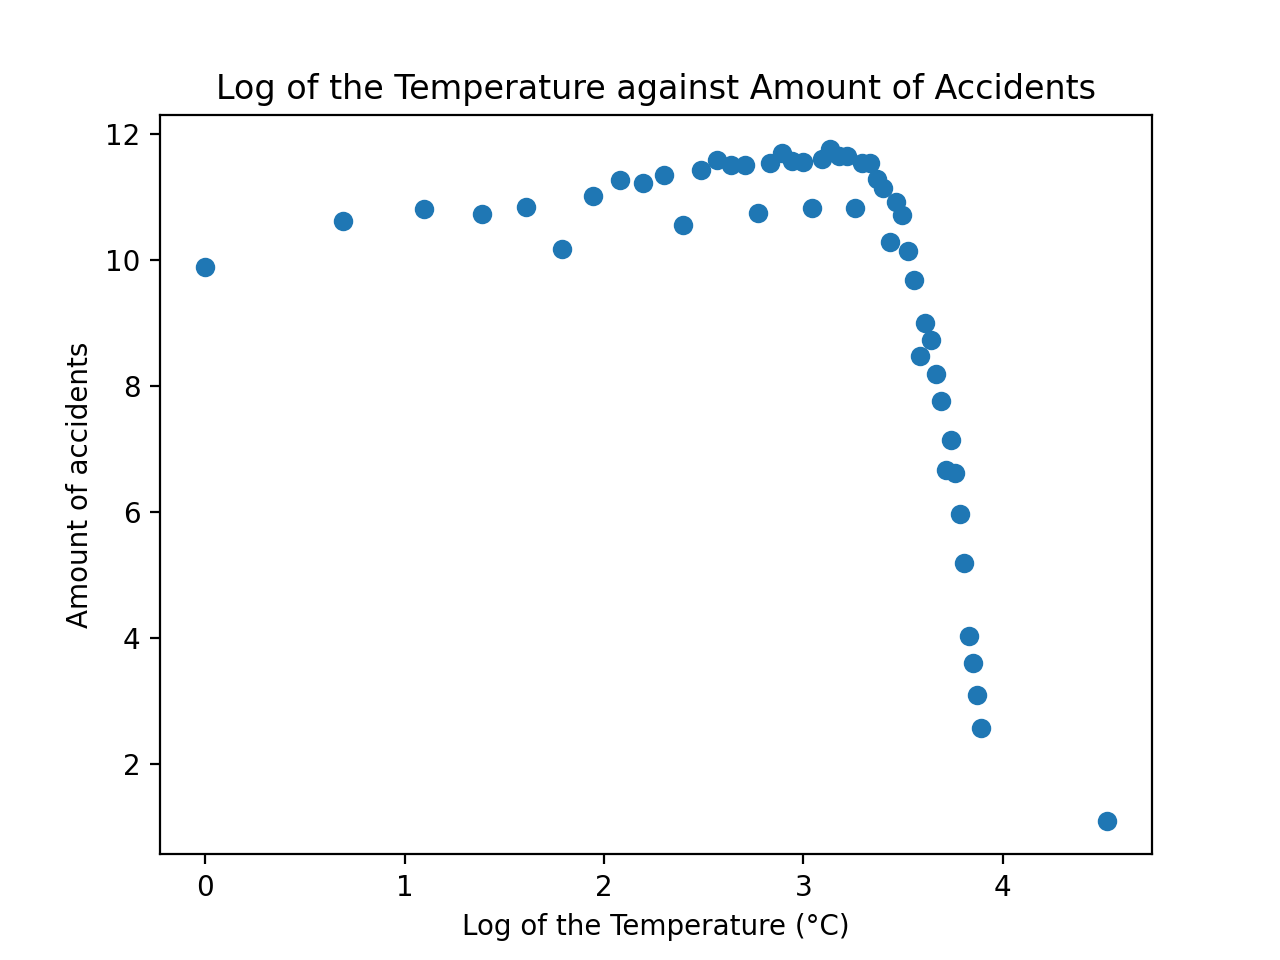
\includegraphics[scale=0.5]{../figures/highres/log_temperature_against_amount_of_accidents.png}
    \caption{Log of the Amount of Car Accidents vs. Temperature in the US}
    \label{fig:usa_log_accidents_vs_temp}
\end{figure}

The inference will then simply have to take the exponential of the prediction to get the actual amount of accidents.

By following this methodology, the research study aimed to investigate the relationship between weather conditions and car accidents, assess the predictive capabilities of the models, and explore the potential of using weather conditions to predict car accidents and mitigate risks associated with adverse weather conditions.

\section{Results and Analysis}

The results and analysis section presents the findings of the study, including the outcomes of the linear regression analysis on the Iceland Dataset and the random forest regression analysis on the USA Dataset.

\subsection{Linear Regression Results (Iceland Dataset)}

The linear regression analysis aimed to examine the relationship between temperature and car accidents using the Iceland Dataset. The results indicate a significant relationship between temperature and car accidents in Iceland. However, due to the limited amount of data available and the presence of considerable variance or noise, the model's performance was affected. Despite these challenges, the model was able to predict the average amount of car accidents per month for the entire country of Iceland.

Table 1 presents the metrics used to evaluate the performance of the linear regression model on the Iceland Dataset:

\begin{table}[htbp]
    \centering
    \caption{Linear Regression Results (Iceland Dataset)}
    \begin{tabular}{lll}
        \hline
        Metric                    & Value                           & Interpretation                  \\
        \hline
        Mean Squared Error (MSE)  & 2128.68                         & Lower is better                 \\
        Mean Absolute Error (MAE) & 39.46                           & Lower is better                 \\
        R-squared Score (R2)      & 0.14                            & Higher is better (1 is highest) \\
        Validation score          & 0.14
                                  & Higher is better (1 is highest)                                   \\
        % Cross-Validation Scores   & [-0.48, -1.15, 0.18, -0.15, -0.30] & Higher is better \\
        \hline
    \end{tabular}
\end{table}




The mean squared error (MSE) of 2128.68 suggests that the model's predictions have a moderate level of error. The mean absolute error (MAE) of 39.46 indicates the average difference between the predicted and actual values of car accidents. The R-squared score (R2) of 0.14 indicates that the model explains 14\% of the variance in the car accidents based on temperature. A validation score of 0.14 suggests that the model's predictive ability for car accidents based on temperature alone may be limited when faced with new temperature data. The relatively low validation score implies that the model does not generalize well to new, unseen data, which can be attributed to the limited amount of available data and the inherent variability in the relationship between temperature and car accidents.

It is worth noting that a higher validation score would have indicated a better ability of the model to generalize to new data. However, with the current findings, it is evident that the linear regression model's predictive power for car accidents in Iceland based solely on temperature is modest, this becomes obvious when plotting the predictions of the model against the actual data See Figure \ref{fig:isl_model}. But, considering the limited amount of data available, and the amount of noise in the data, the model's performance is as good as it gets.

\begin{figure}
    \centering
    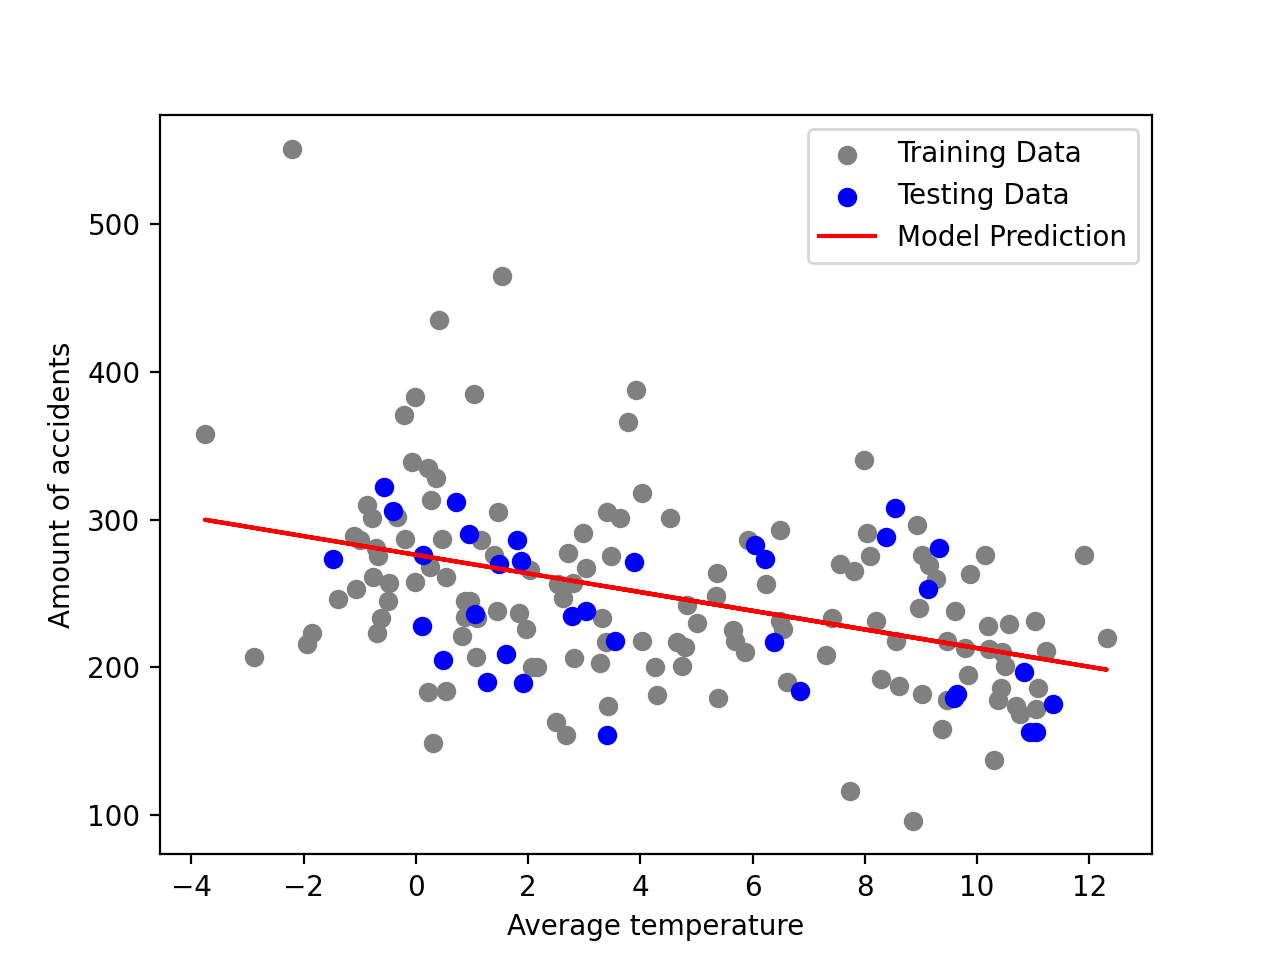
\includegraphics[scale=0.5]{../figures/highres/isl_model.png}
    \caption{Linear Regression Model Predictions vs. Actual Data (Iceland Dataset)}
    \label{fig:isl_model}
\end{figure}

% The cross-validation scores further support the model's performance, with higher values indicating a better fit.

\subsection{Random Forest Regression Results (USA Dataset)}

The random forest regression analysis aimed to predict car accidents based on temperature and wind speed using the USA Dataset. The results showed a significant relationship between temperature and car accidents, while wind speed did not exhibit a significant relationship with car accidents across the entire USA dataset. This can be attributed to the fact that not all accidents are influenced by wind speed, and the majority of accidents occur in urban areas where wind speed is less likely to be a contributing factor.

Table 2 presents the metrics used to evaluate the performance of the random forest regression model on the USA Dataset:

\begin{table}[htbp]
    \centering
    \caption{Random Forest Regression Results (USA Dataset)}
    \begin{tabular}{ccc}
        \hline
        Metric                    & Value        & Interpretation                  \\
        \hline
        Mean Squared Error (MSE)  & 394824074.01 & Lower is better                 \\
        Mean Absolute Error (MAE) & 10451.87     & Lower is better                 \\
        R-squared Score (R2)      & -0.38        & Higher is better (1 is highest) \\
        Validation score          & 0.96         & Higher is better (1 is highest) \\
        \hline
    \end{tabular}
\end{table}

The model has an impressive validation score of 0.96. This indicates that the random forest model demonstrates a high level of generalization to new, unseen data. With a validation score of 0.96, the model shows a strong ability to predict the average amount of car accidents per month for the entire USA based on temperature and wind speed.

Despite the relatively high mean squared error (MSE) and mean absolute error (MAE), the model is able to accurately predict the average amount of car accidents per month for the entire USA with a high degree of accuracy. It is important to note that while the MSE and MAE reflect the average difference between predicted and actual values, the validation score provides an overall measure of the model's ability to make accurate predictions. In this case, the high validation accuracy suggests that the model is effectively capturing the underlying patterns and relationships between temperature, wind speed, and car accidents in the USA dataset.

The R-squared score (R2) of -0.38 indicates that the model explains a limited amount of variance in the car accidents based on temperature and wind speed. A higher R-squared score would indicate a better fit of the model to the data. Therefore, the model may not capture all the factors influencing car accidents accurately, as indicated by the relatively low R-squared score.

However, when plotting the predictions of the model against the actual data, it is evident that the model is able to capture the underlying patterns and relationships between temperature, wind speed, and car accidents in the USA dataset See Figure \ref{fig:usa_model}. In the figure the model predicts that the amount of accidents increases in high wind speeds and both extremes of the temperature

\begin{figure}
    \centering
    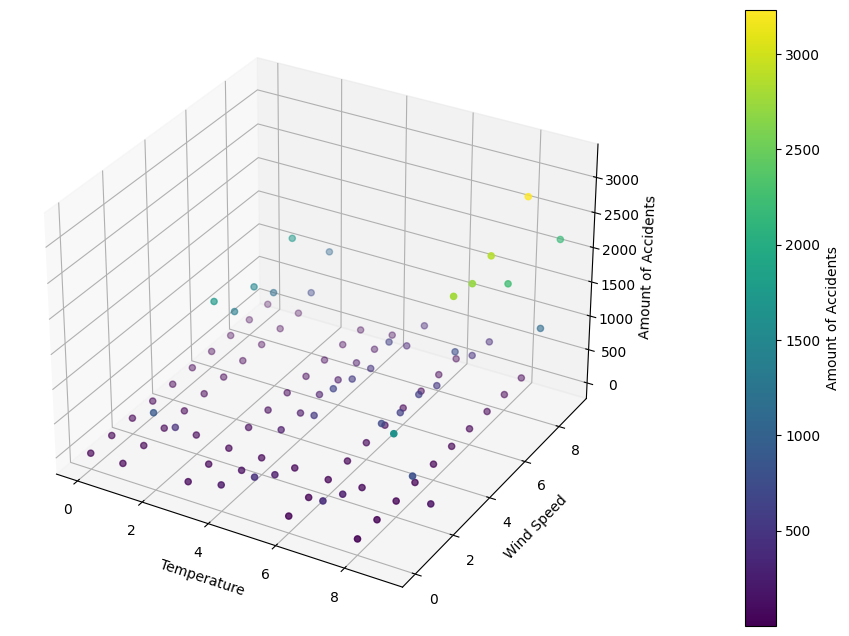
\includegraphics[scale=0.5]{../figures/highres/usa_model.png}
    \caption{Random Forest Regression Model Predictions vs. Actual Data (USA Dataset). The scale of the temperature is between 0 and 10, 0 being the coldest(less than -5°C) and 10 being the hottest(more than 35°C), the scale of the wind speed is between 0 and 10, 0 being no wind and 10 being the windiest(more than 20 m/s)}
    \label{fig:usa_model}
\end{figure}

Viewing the same graph, but on only the temperature  and the wind speed axis and taking the average over the other, it is evident that the model is able to capture the underlying patterns and relationships between temperature and car accidents in the USA dataset (See Figure \ref{fig:usa_model_2d}). In the figure the model predicts that the amount of accidents increases in both extremes of the temperature, the same for the wind speed. Except, when asked to predict the amount of accidents in winds higher than "High" or in wind speeds grater than 14 m/s. This can be explained by the fact that the model has not seen as much data with such high wind speeds, and therefore, it is not able to predict the amount of accidents in such conditions.

\begin{figure}
    \centering
    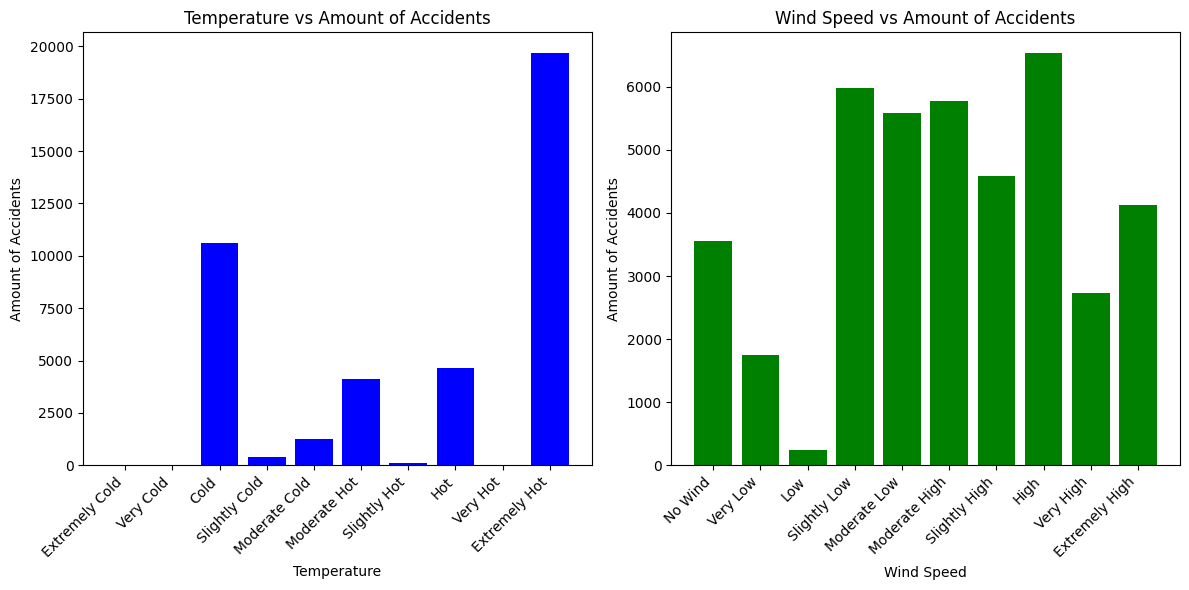
\includegraphics[scale=0.4]{../figures/highres/usa_model_2d.png}
    \caption{Random Forest Regression Model Predictions vs. Actual Data (USA Dataset). Viewed on only the temperature  and the wind speed axis. Extremely cold temperatures are less than -5°C, extremely hot temperatures are more than 35°C, no wind is less than 5 m/s and extremely high wind speed is more than 20 m/s, the scale is linear}
    \label{fig:usa_model_2d}
\end{figure}


Overall, the random forest regression model demonstrates strong generalization capabilities to new data. However, further analysis and consideration of additional factors may be required to improve the model's ability to explain a larger proportion of the variance in car accidents and enhance its predictive accuracy.

\newpage
\section{Discussion}

The discussion section of this research paper highlights the study's limitations and proposes future research directions. It is important to consider these limitations when interpreting the findings.

One limitation is that the analysis focused solely on the relationship between temperature and car accidents, neglecting other variables that may influence accident rates, such as rainfall, snowfall, road conditions, visibility, and driver behavior. Incorporating these variables in future research would provide a more comprehensive understanding and improve predictive models.

Another limitation is the limited amount of data available for the study, which focused on Iceland. To enhance generalizability, future studies should expand the dataset by including data from multiple regions with diverse weather conditions and driving environments.

Additionally, the findings may not be applicable on a global scale since the datasets used were specific to Iceland. Future research should consider incorporating datasets from different geographical regions to capture global patterns and gain a more comprehensive understanding of the relationship between weather conditions and car accidents worldwide.

Future work should include the inclusion of additional variables, expansion to different geographical regions and diverse weather conditions, and longitudinal studies covering extended periods. Utilizing advanced modeling techniques, such as machine learning algorithms, can also enhance the accuracy of predictive models and uncover complex relationships.

By addressing these limitations and pursuing the suggested future research directions, researchers can contribute to a comprehensive understanding of the relationship between weather conditions and car accidents. This knowledge can inform the development of effective strategies for accident prevention, road safety measures, and weather-based warning systems, ultimately promoting safer driving practices and reducing the frequency and severity of car accidents.


\section{Conclusion}

In conclusion, this research study aimed to investigate the feasibility of predicting the average amount of car accidents in Iceland based on current weather conditions. Despite the limitations of the available data and the absence of wind speed information for Iceland, the study provided valuable insights into the relationship between weather conditions and car accidents.

The findings emphasize the potential of utilizing weather conditions to predict car accidents and enhance road safety. By incorporating additional variables, expanding geographical coverage, and employing advanced modeling techniques, future research can further improve predictive models and uncover complex relationships between weather conditions and car accidents.

The limitations of this study, including the focus on temperature as the sole weather variable and the limited dataset availability, should be considered when interpreting the findings. Future research should incorporate other influential variables, encompass diverse geographical regions, and conduct longitudinal studies to capture long-term trends and temporal patterns.

Overall, this research contributes to the understanding of the relationship between weather conditions and car accidents, paving the way for the development of proactive strategies to enhance road safety. By leveraging predictive models and weather-based warning systems, it becomes possible to mitigate risks associated with adverse weather conditions, promote safer driving practices, and ultimately reduce the frequency and severity of car accidents.

\bibliography{references}
\bibliographystyle{plain}

\end{document}